In subsection~\ref{subsec:E-L-optimization} we expressed some concerns about the result obtained in~\eqref{eq:minimized-V-beta}, and outlined a procedure to compute a more sophisticated bound.
As anticipated, we would like to write an Euler-Lagrange equation for the functional \(J\), whose solution would represent its minimal point.
However, we have already seen in~\ref{sec:comparison-2-methods} that the Euler-Lagrange equation associated to \(J\) is nothing else than the Raychaudhuri's equation; reducing directly to that would bring all the complications already discussed due to the presence of the Ricci tensor, and this would take us no further.

The idea is then to apply the energy conditions \emph{before} computing the Euler-Lagrange equation, but unfortunately this cannot be done directly because the Sobolev energy conditions are applicable to a set of functions different from the one onto which we want to run the minimization.

Let us reduce to a little easier problem, and try to minimize \(J\) on
\[
\mathcal{A}_{E.L.} \coloneqq \{f \quad \vert \quad \exists \ell_0 > 0 \text{ s.t. } f(\lambda \le \ell_0) \equiv 1\} \supset \mathcal{A}_{\beta}
\]
instead of the most general set, again in a variational spirit.

To overcome the difficulties in applying the energy conditions, we need the help of some auxiliary function \(\varphi\) such that:
\[
\varphi(\lambda \ge \ell_0) \equiv 1 \implies \left(\varphi f\right)   =
\begin{cases}
    0 \text{ at } \lambda = 0;\\
    0 \text{ at } \lambda = \ell.
\end{cases}
\]
This way the product \(\varphi f\) belongs to the set of functions to which the Sobolev energy condition can be applied; moreover we still have the helpful identity \(f^2 = \left(\varphi f\right)^2 + \left(1 - \varphi^2\right) f^2 = \left(\varphi f\right)^2 + \left(1 - \varphi^2\right)\). The idea is then to write two separate Euler-Lagrange equations in order to determine both the best \(\varphi\) and \(f\). 
% \begin{wrapfigure}{l}{0.5\textwidth}
%     \centering
%     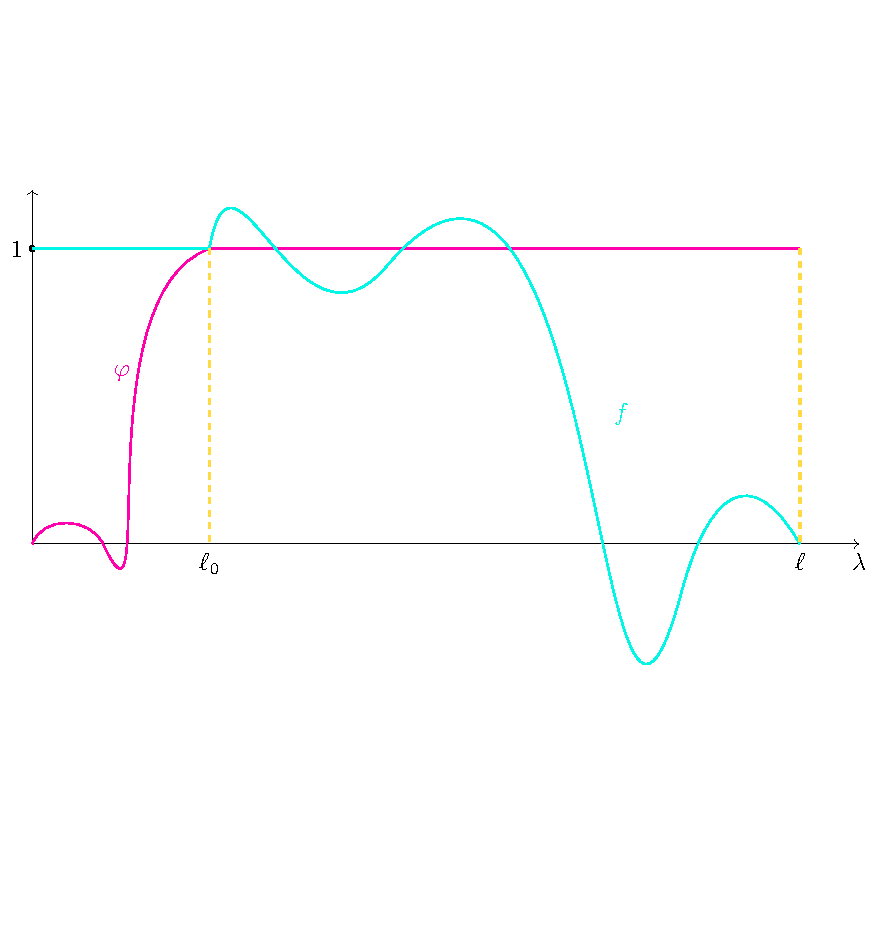
\includegraphics[scale=0.4]{Immagini/euler-lagrange-functions/euler-lagrange-functions.pdf}
%     \caption[]{plot of some possible functions \(f\) and \(\varphi\) included in our analysis. The idea is to separately optimize the behaviour of \(\varphi\) before \(\ell_0\), and of \(f\) between \(\ell_0\) and \(\ell\).}
% \end{wrapfigure}

\begin{SCfigure}
    \centering
    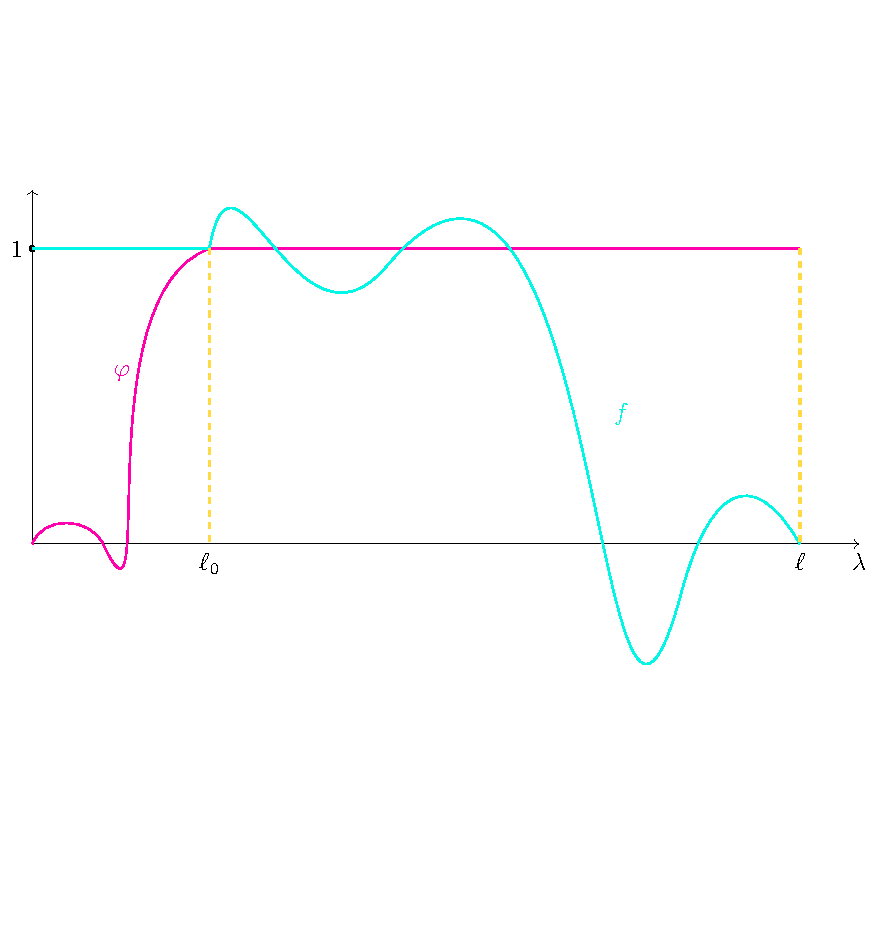
\includegraphics[scale=0.6]{Immagini/euler-lagrange-functions/euler-lagrange-functions.pdf}
    \caption[]{plot of some possible functions \(f\) and \(\varphi\) included in our analysis. The idea is to separately optimize the behaviour of \(\varphi\) before \(\ell_0\), and of \(f\) between \(\ell_0\) and \(\ell\).}
\end{SCfigure}
We can write\footnote{we specialize to the case of Sobolev conditions with \(m = 1\); the same procedure could be generalized at the price of facing higher order differential equations.}
\begin{align*}
    J[f] &= (n - 2)\vert\vert\nabla_U f \vert\vert^2 - \int_0^{\ell} R_{\mu\nu}U^{\mu}U^{\nu} f^2 d\lambda =\\
    &= (n - 2)\vert\vert\nabla_U f \vert\vert^2 - \int_0^{\ell} R_{\mu\nu}U^{\mu}U^{\nu} \left(\varphi f\right)^2 d\lambda - \int_0^{\ell} \left(1 - \varphi^2\right) R_{\mu\nu}U^{\mu}U^{\nu} d\lambda \le \\
    &\le (n - 2)\vert\vert\nabla_U f \vert\vert^2 + Q_0\vert\vert\varphi f\vert\vert^2 + Q_1\vert\vert\left(\varphi f\right)'\vert\vert^2 - \int_0^{\ell_0} \left(1 - \varphi^2\right) R_{\mu\nu}U^{\mu}U^{\nu} d\lambda.
\end{align*}
Now, the problem separates because
\begin{align*}
    \vert\vert\varphi f\vert\vert^2 &= \int_0^{\ell} \left(\varphi f\right)^2 d\lambda = \underbrace{\int_0^{\ell_0}\varphi^2d\lambda}_{\vert\vert\varphi \vert\vert_{\ell_0^-}^2} + \underbrace{\int_{\ell_0}^{\ell}f^2d\lambda}_{\vert\vert f \vert\vert_{\ell_0^+}^2} \\
    \vert\vert\left(\varphi f\right)'\vert\vert^2 &= \int_0^{\ell} \left(\varphi' f\right)^2 d\lambda +\int_0^{\ell} \left(\varphi f'\right)^2 d\lambda + 2 \int_0^{\ell} \varphi\cdot f\cdot \underbrace{\varphi'\cdot f'}_{0}d\lambda = \\
    &= \underbrace{\int_0^{\ell_0}\varphi'^2d\lambda}_{\vert\vert\varphi '\vert\vert_{\ell_0^-}^2} + \underbrace{\int_{\ell_0}^{\ell}f'^2d\lambda}_{\vert\vert f' \vert\vert_{\ell_0^+}^2}.
\end{align*}
And finally, if we assume again \(0 \ge R_{\mu\nu}U^{\mu}U{\nu} \ge - \vert\rho_0\vert\) 
\[
\varphi^2 \ge 0 \implies 1 - \varphi^2 \le 1 \implies \int_0^{\ell_0} \left(1 - \varphi^2\right) R_{\mu\nu}U^{\mu}U^{\nu} d\lambda \ge -\vert\rho_0\vert \ell_0,    
\]
we obtain
\[
J[f] \le K[f] \coloneqq \left[n - 2 + Q_1\right] \vert\vert\nabla_U f \vert\vert_{\ell_0^+}^2 + Q_0\vert\vert f \vert\vert_{\ell_0^+}^2 + Q_1 \vert\vert\varphi '\vert\vert_{\ell_0^-}^2 + Q_0\vert\vert\varphi\vert\vert_{\ell_0^-}^2 + \vert\rho_0\vert \ell_0.
\]
The Euler-Lagrange equations for the functional \(K\) are:
\begin{align*}
    f '' = \frac{Q_0}{n -2 + Q_1}f \quad\quad &f(\ell_0) = 1 \quad f(\ell) = 0,\\
    \varphi'' = \frac{Q_0}{Q_1}\varphi \quad\quad &\varphi(0) = 0 \quad \varphi(\ell_0) = 1,
\end{align*}
that have unique solution
\begin{align*}
    f(\lambda) &= \sinh\left[\Omega_1(\lambda - \ell_0)\right]-\coth\left[\Omega_1(\ell - \ell_0)\right]\cdot\cosh\left[\Omega_1(\lambda - \ell_0)\right] \\
    \varphi(\lambda) &= \frac{1}{\sinh\left[\Omega_2\ell_0\right]} \cdot \sinh\left[\Omega_2\lambda\right],
\end{align*}
where, \(\coth x\) is the hyperbolic cotangent, and for convenience we have defined:
\[
\Omega_1^2 \coloneqq \frac{Q_0}{n - 2 + Q_1} \quad \quad  \Omega_2^2 \coloneqq \frac{Q_0}{Q_1}.
\]
As it has been already pointed out in~\ref{sec:comparison-2-methods}, for functionals such as \(K\), if \(f\) and \(\varphi\) are the optimal functions, then the minimal point is simply:
\begin{align*}
    K[f, \varphi] &= \int_{\ell_0}^{\ell}\left\{\left[n - 2 + Q_1\right] f'(\lambda)^2  + Q_0 f(\lambda)^2\right\}d\lambda + \\
    &+\int_{0}^{\ell_0}\left\{Q_1 \varphi'(\lambda)^2  + Q_0 \varphi(\lambda)^2\right\}d\lambda + \vert\rho_0\vert\ell_0 = \\
    &= \left[n - 2 + Q_1\right] f'\cdot f\Big\vert_{\ell_0}^{\ell} + \int_{\ell_0}^{\ell} f\underbrace{\left\{Q_0f - \left(n - 2 + Q_1\right)f''\right\}}_{0} d\lambda + \\ &+ Q_1\varphi\varphi'\Big\vert_0^{\ell_0} + \int_{0}^{\ell_0} \varphi\underbrace{\left\{Q_0f -  Q_1\varphi''\right\}}_{0} d\lambda + \vert\rho_0\vert\ell_0 =\\
    &=-\left[n - 2 + Q_1\right] f'(\ell_0) +Q_1\varphi'(\ell_0) + \vert\rho_0\vert\ell_0 = \\
    &= \sqrt{Q_0(n - 2 + Q_1)}\coth\left[\Omega_1(\ell- \ell_0)\right] + \sqrt{Q_0Q_1}\coth\left[\Omega_2\ell_0\right] + \vert \rho_0\vert\ell_0 = \\
    &\coloneqq \mathcal{V}_{E.L.}(\ell_0, \ell).
\end{align*}
This means we have proved that:
\[
    \inf_{\substack{f\in C^{\infty}_{1,0}[0, \ell]\\ \ell > 0}}J_{\ell}[f] \le \mathcal{V}_{E.L.}(\ell_0, \ell)
\]
where \(\mathcal{V}_{E.L.}(\ell_0, \ell)\) can be found in~\eqref{eq:V-euler-lagrange}. 
For the sake of completeness we include a comparison between the \(2\) minimal functions derived above, and the \(14-\)incomplete beta function.
\begin{figure}
    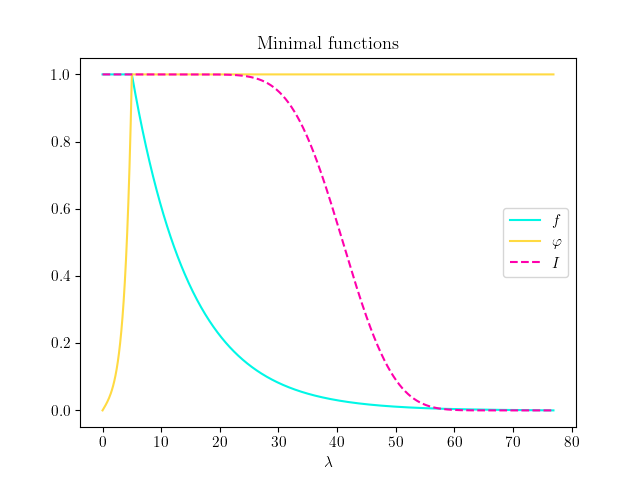
\includegraphics[scale=0.9]{Immagini/minimal-functions.png}
    \caption[]{\(f\) and \(\varphi\) are the functions that minimize the functional \(K\) as defined above. \(I\) is the \(14\)-incomplete beta function, belonging to the set \(\mathcal{A}_{\beta} \subset \mathcal{A}_{E.L.}\) onto which we have minimized \(J\) in section~\ref{subsec:V-optimization}.}
\end{figure}